\chapter{Introducción específica} % Main chapter title
\label{Chapter2}
%----------------------------------------------------------------------------------------
%	SECTION 1
%----------------------------------------------------------------------------------------
En este capítulo se presentan los requerimientos acordados con el cliente y los recursos de hardware (HW) y software (SW) utilizados para el desarrollo de trabajo. Se describen en las partes implementadas del HW, los servicios integrados de backend (BES) y solamente algunos aspectos relevantes del firmware (FW) que interactúa con el hardware. En el capítulo 3 se abarca la lógica de negocios implementada en el FW del microcontrolador.\\
\section{Requerimientos acordados con el cliente}
\label{sec:requerimientos}
\begin{enumerate}
	\item Grupo de requerimientos asociados con hardware
	\begin{enumerate}
		\item El dispositivo deberá ser de tipo \textit{plug and play}.
		\item El circuito impreso no deberá ocupar un volumen mayor a 10x10x5 cm.
		\item Basarse en un microcontrolador ESP32 y disponer de:
		\begin{enumerate}%[label*=\arabic*.]
			\item 4 entradas analógicas.
			\item 3 salidas digitales.
			\item Unidad UART.
			\item Integrar un módulo de comunicaciones LoRa.
		\end{enumerate}
		\item Deberá tener al menos 12 horas de autonomía de funcionamiento.
		\item Bajo consumo en modo ocioso: el consumo del hardware en total, no deberá superar los 5 mA cuando no está midiendo ni transmitiendo.
		\item El circuito elevador de tensión DC-DC deberá:
		\begin{enumerate}%[label*=\arabic*.]
			\item Funcionar con tensiones menores a 2V en la entrada.
			\item Otorgar 5 Volts a la salida.
			\item Ser capaz de otorgar 300 miliamperes a la salida.
		\end{enumerate}
		\item El transformador de corriente debe:
		\begin{enumerate}%[label*=\arabic*.]
			\item Ser de tipo núcleo partido.
			\item Admitir 100 Amperes de corriente en el circuito primario y un máximo 5 Amperes en el circuito secundario.
		\end{enumerate}
		\item \label{req_relay} El relay encargado de cambiar el modo de operación debe:
		\begin{enumerate}%[label*=\arabic*.]
			\item Ser de tipo doble invesor sin retención.
			\item Su bobina debe poder energizarse con 5V o menos.
			\item Soportar al menos 5 Amperes de corriente por los contactos.
		\end{enumerate} 
		\item Debe funcionar de manera independiente a la frecuencia de operación de la red 50/60 Hz.
		\item Debe funcionar de manera independiente a la tensión de fase del sistema de distribución 110/220 Voltios.
	\end{enumerate}
	\item Grupo de requerimientos asociados con el firmware
	\begin{enumerate}
		\item Debe manejar un módulo de comunicación LoRa y protocolo LoRaWAN.
		\item Deberá tener un porcentaje de cobertura de tests unitarios del 60\% como mínimo.
		\item Antes configurarse en modo ocioso, debe desenergizar la etapa de medición de corriente y el módulo de comunicaciones con el objeto de ahorrar energía.
	\end{enumerate}
	
	\item Grupo de requerimientos asociados con los BES
	\label{requerimientos_backend}
	\begin{enumerate}
		\item Todos los servicios deben poder correr en una Raspberry Pi 3.
		\item El software de los BES se desarrollará en lenguaje Python.
		\item Recuperar los datos de la red LoRaWAN.\label{requerimiento_LORAWAN}
		\item Almacenar los datos en una tabla de MySQL.
		\item GUI basada en Grafana.
	\end{enumerate}
	
	\item Grupo de requerimientos asociados con ensayos de integración y \textit{end-to-end}
	\begin{enumerate}
		\item El banco de ensayos de hardware debe contar con una carga fantasma de al menos 10 Amperes y permitir realizar interrupciones de corriente de manera programada mediante una computadora adicional tipo Raspberry Pi o de manera manual.
		\item Los BES deben estar operativos al momento de realizar los ensayos.
		\item Contar con un gateway de acceso a una red LoRaWAN como por ejemplo \textit{The Things Network}.
	\end{enumerate}
\end{enumerate}


\section{Diagrama de bloques general del sistema implementado}
El diagrama de bloques del HW a instalar \textit{in situ} es presentado en la figura \ref{fig:diagramadebloquesdelhw} y consta de cuatro bloques:
% TODO: \usepackage{graphicx} required
\begin{figure}[h!]
	\centering
	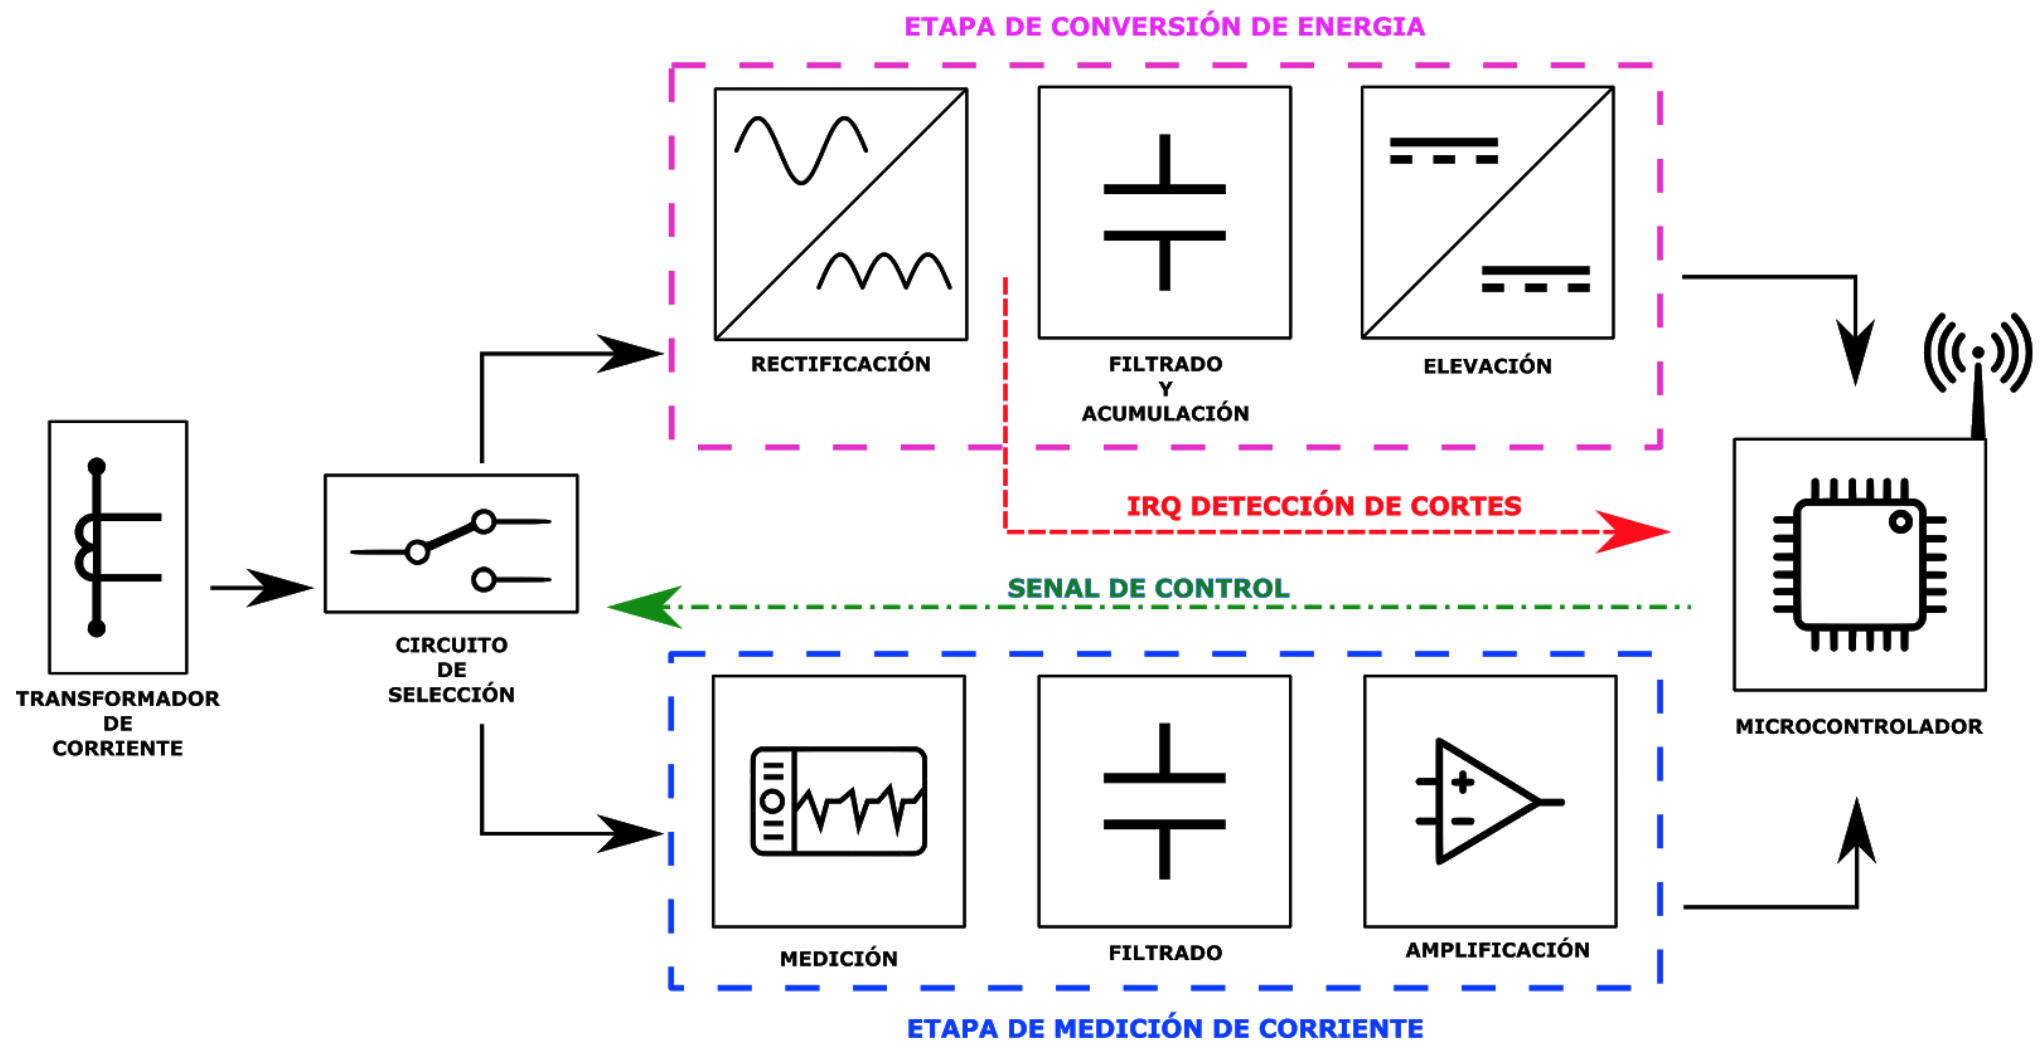
\includegraphics[width=0.9\linewidth]{Figures/diagrama_de_bloques_del_HW}
	\caption{Diagrama de bloques del HW para el nodo a instalar \textit{in situ}}
	\label{fig:diagramadebloquesdelhw}
\end{figure}
\begin{enumerate}
	\item Circuito de selección de modo: un relay (RL) y su circuito de mando controlarán a que etapa del nodo se conectarán los terminales del TI.
	\item Etapa de rectificación, acumulación de energía y elevación de tensión: compuesta por rectificador de onda completa, una etapa de filtrado y acumulación y un circuito elevador de tensión.
	\item Etapa de medición de valor RMS de corriente: un chip dedicado toma la señal de tensión generada en bornes del resistor shunt y calcula el valor RMS. A su salida entrega un valor proporcional de tensión DC.
	\item Microcontrolador (MC): ejecutar la lógica de negocios que rige el comportamiento del nodo, digitalizar mediciones y transmitir datos a la red LoRaWAN.
\end{enumerate}
Por otro lado, el sistema también implica el desarrollo y puesta en funcionamiento de un conjunto de servicios de \textit{backend} (BES) propios del proyecto que cumplen las funciones de:
\begin{itemize}
	\item Recuperación de datos de la red LoRaWAN.
	\item Almacenamiento en una base de datos (DB).
	\item Presentación de los datos al usuario final mediante una interfaz gráfica de usuario (GUI).
\end{itemize}
% TODO: \usepackage{graphicx} required
\begin{figure}[h]
	\centering
	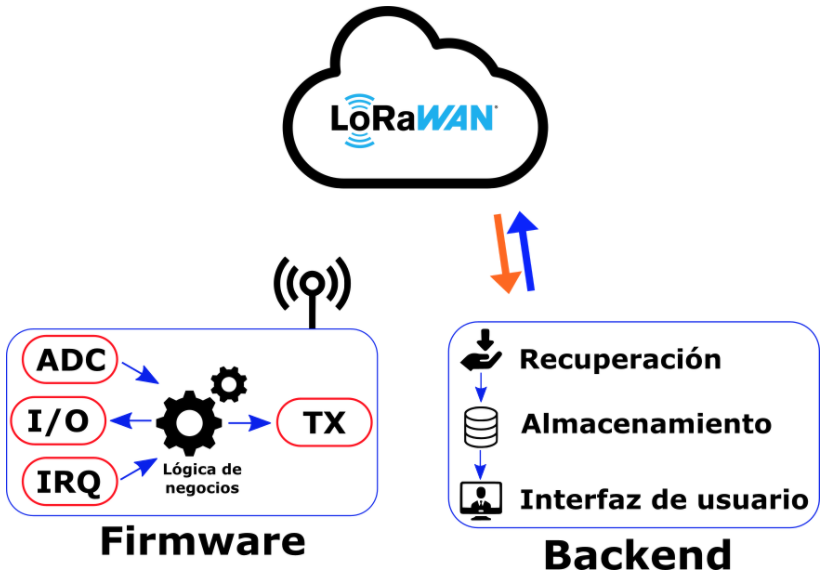
\includegraphics[width=0.7\linewidth]{Figures/diagrama_de_bloques_de_BES}
	\caption{Diagrama de bloques del FW implementado en el MC y su interacción con la red LoRaWAN y los BES privados del sistema.}
	\label{fig:diagramadebloquesdebes}
\end{figure}
El requisito \ref{requerimiento_LORAWAN} impuso el uso de una red LoRaWAN como columna vertebral para la transmisión de datos generados por los nodos. Para cumplirlo se adoptó la arquitectura presentada en la figura \ref{fig:diagramadebloquesdebes}.
Las mediciones son tomadas por el HW y transmitidas hacia la red LoRaWAN para luego interactuar con los BES privados que se encargan de recuperar, almacenar y presentar los datos al usuario final.
Una interfaz gráfica de como la presentada en la figura \ref{fig:guirequeridaporelcliente}, se encarga de presentar al usuario final los últimos datos adquiridos por cada nodo. De esta manera, se puede identificar de manera simple mediante un punto verde o rojo sobre el mapa si la línea monitoreada presenta un problema.
% TODO: \usepackage{graphicx} required
\begin{figure}[h]
	\centering
	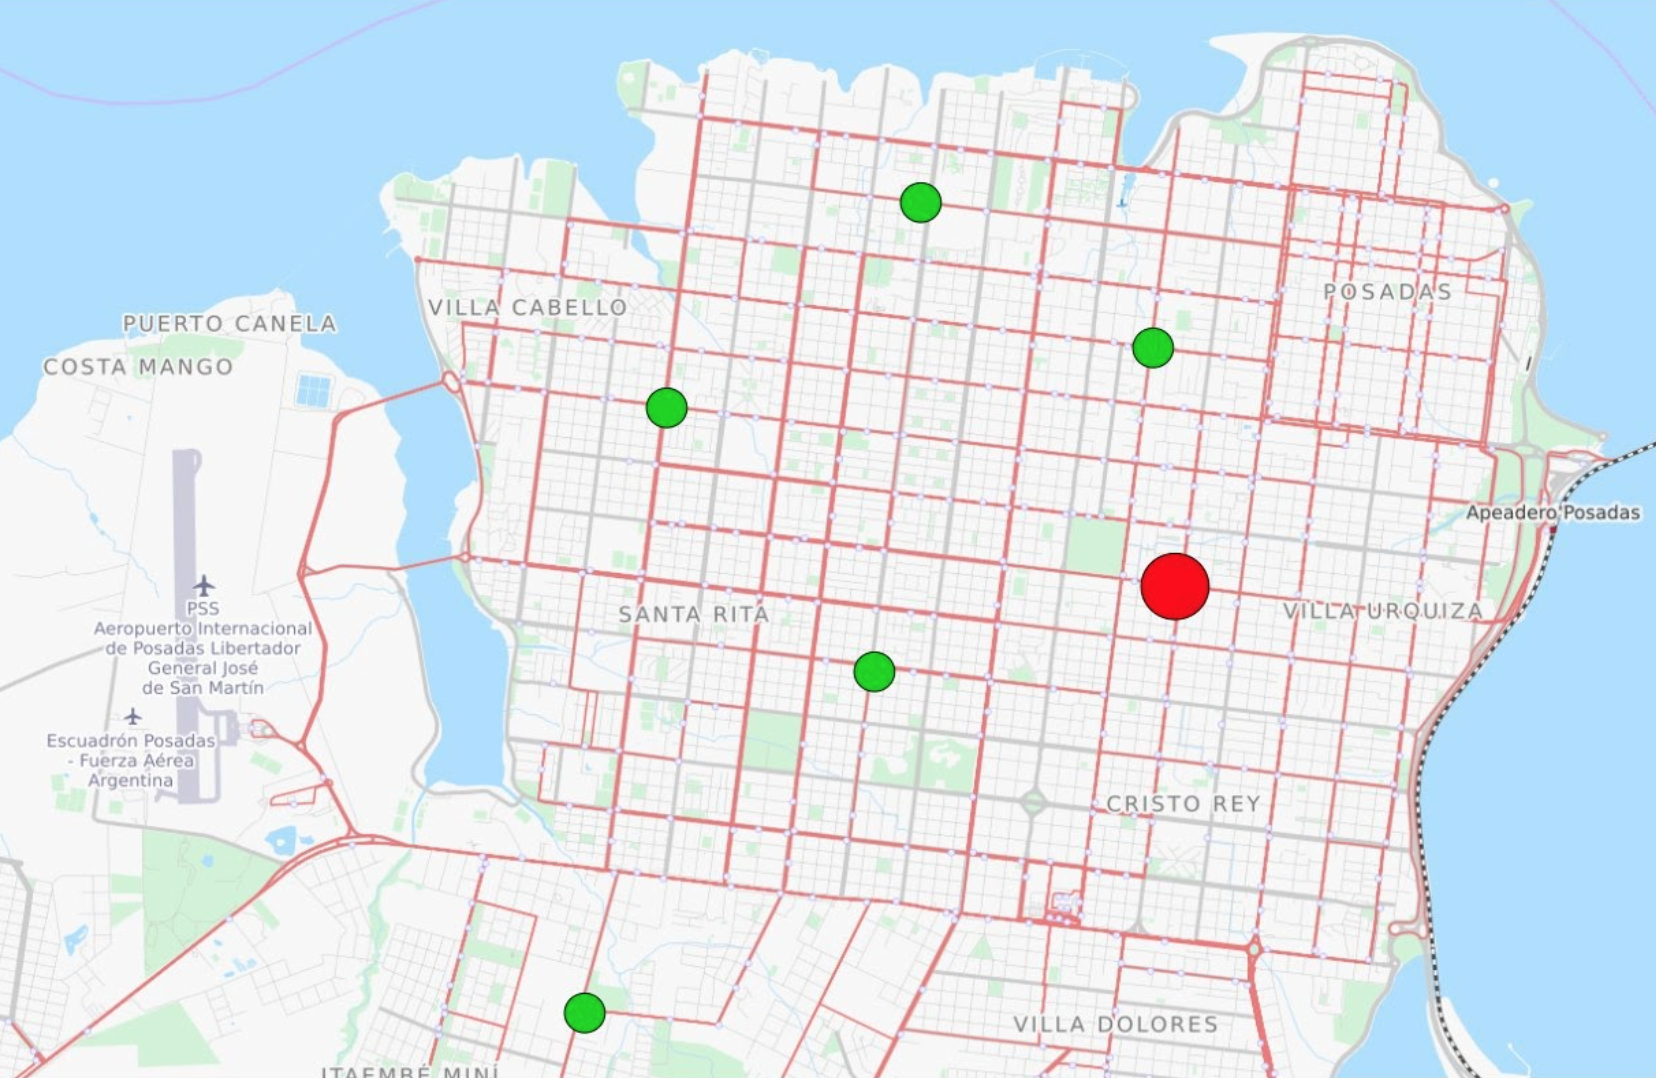
\includegraphics[width=0.7\linewidth]{Figures/GUI_requerida_por_el_cliente}
	\caption{Ejemplo de interfaz gráfica de usuario requerida por el cliente para presentar los últimos datos recuperados por cada nodo en la ciudad de Posadas, Misiones.}
	\label{fig:guirequeridaporelcliente}
\end{figure}

\section{Detalle del hardware}
\subsection{Transformador de corriente}
% TODO: \usepackage{graphicx} required
\begin{figure}[h]
	\centering
	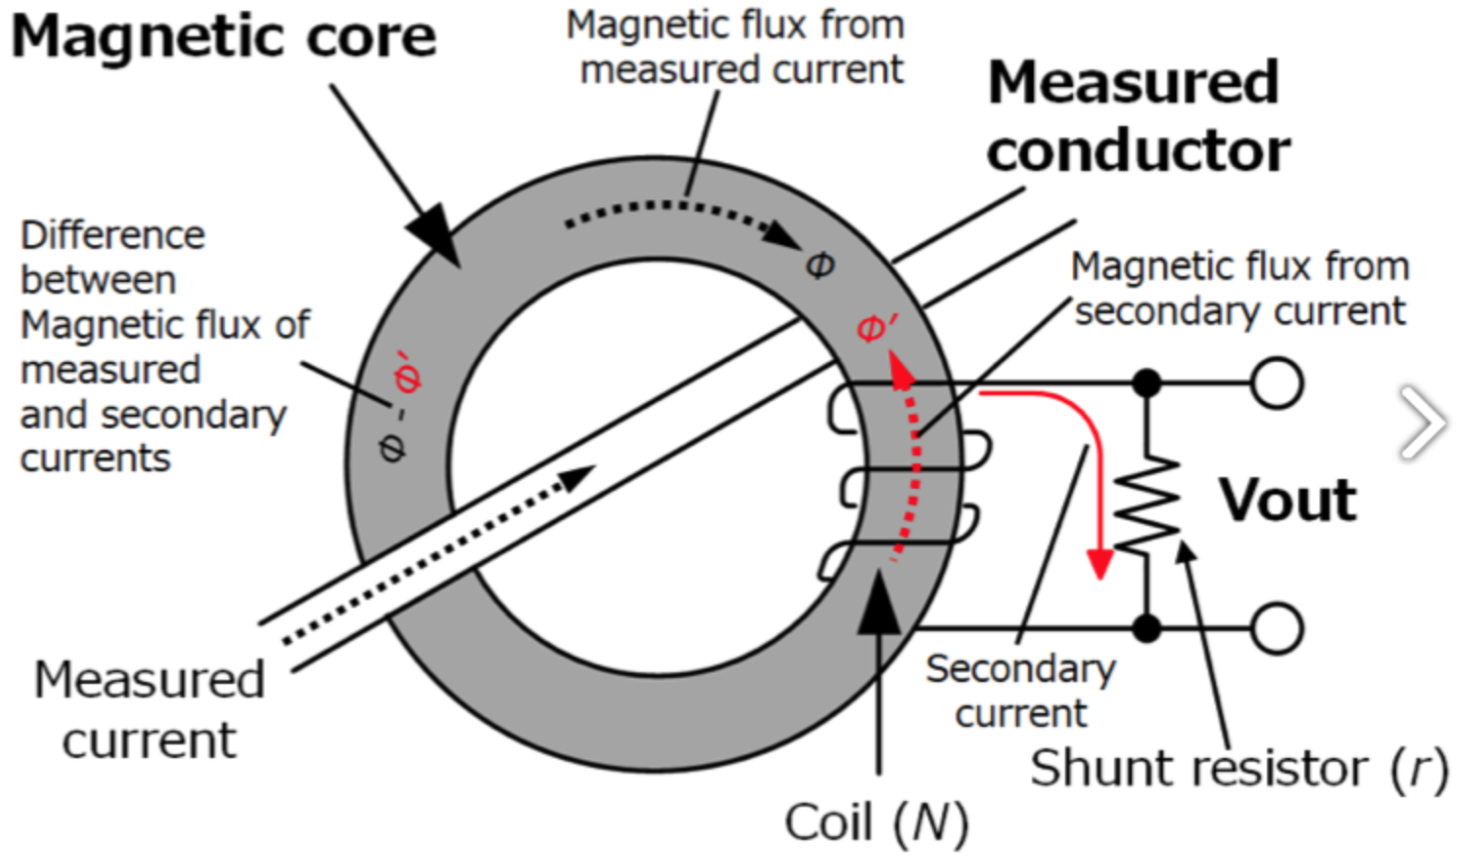
\includegraphics[width=0.7\linewidth]{Figures/dibujo_medicion_TI}
	\caption{Circuito de medicion indirecta de corriente mediante un TI.\citep{hioki}}
	\label{fig:dibujomedicionti}
\end{figure}

\subsection{Circuito de selección}
A partir del lineamiento de que el TI debe estar conectado a la entrada del rectificador por defecto y al resistor shunt al energizarse la bobina del RL, el número y la disposición de los contactos fue un factor relevante al momento de elegir la mejor opción. La variante comercial que cumplió con los requisitos \ref{req_relay} es la producida por la firma Hongfa modelo HF115F/005-2ZS4A presentada en la figura \ref{fig:relay}.
\begin{figure}[h!]
    \centering
	\begin{subfigure}[b]{0.3\textwidth}
		\centering
		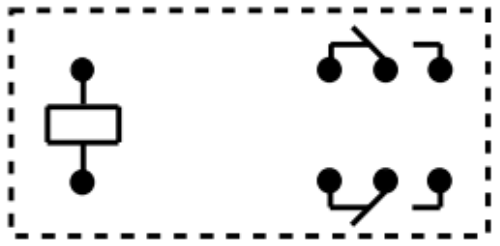
\includegraphics[width=.65\textwidth]{./Figures/relay_pinout}
		\caption{}
		\label{fig:relay_pinout}
	\end{subfigure}
    \centering
	\begin{subfigure}[b]{0.3\textwidth}
		\centering
		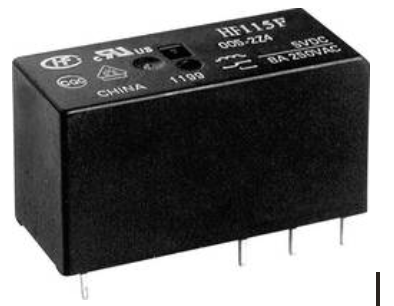
\includegraphics[width=.65\textwidth]{./Figures/relay_encapsulado}
		\caption{}
		\label{fig:relay_encapsulado}
	\end{subfigure}
	\caption{Pinout del relay HF115F/005-2ZS4A (izquireda) y su encapsulado (derecha). Imágenes tomadas de \citep{datasheet_relay}}
	\label{fig:relay}
\end{figure}

\subsection{Conversión de energía}
Para obtener una tensión continua a partir una alterna generada por el TI, es necesario implementar un puente rectificador de onda completa.\\
En la actualidad la mayoria de los circuitos rectificadores de onda completa se basan en diodos de silicio de bajo costo. Sin embargo, un diodo de silicio posee una caída de tensión tipica de 0,7 V. Esta caída de tension se traduce en pérdidas por efecto Joule y es relevante en dispositivos donde la conversión, acumulación y gestión de energía es critica. Por lo tanto, se desea maximizar la transferencia de tensión y potencia entre entrada y salida del puente rectificador.\\
(Yilmaz, Mehmet) analiza técnicas de rectificación de onda completa con diferentes tipos de diodos, como así también un arreglo de transistores MOSFET pasivo y activo. Las caídas de tensión simuladas entre la entrada y salida entre un puente rectificador de diodos de silicio y uno pasivo basado en MOSFETs se comparan en la figura \ref{fig:comparacion_diodos_vs_MOSFET}.\\
Al comparar las simulaciones expuestas en las figuras \ref{fig:onda_rectificador_diodos} y \ref{fig:onda_rectificador_MOSFET} se aprecia que la caída de tensión generada por el rectificador basado en MOSFET al entrar en conducción es menor que uno hecho con diodos, por lo tanto también la potencia disipada en forma de calor.\\
\begin{figure}
	\begin{subfigure}{.5\textwidth}
		\centering
		% include first image
		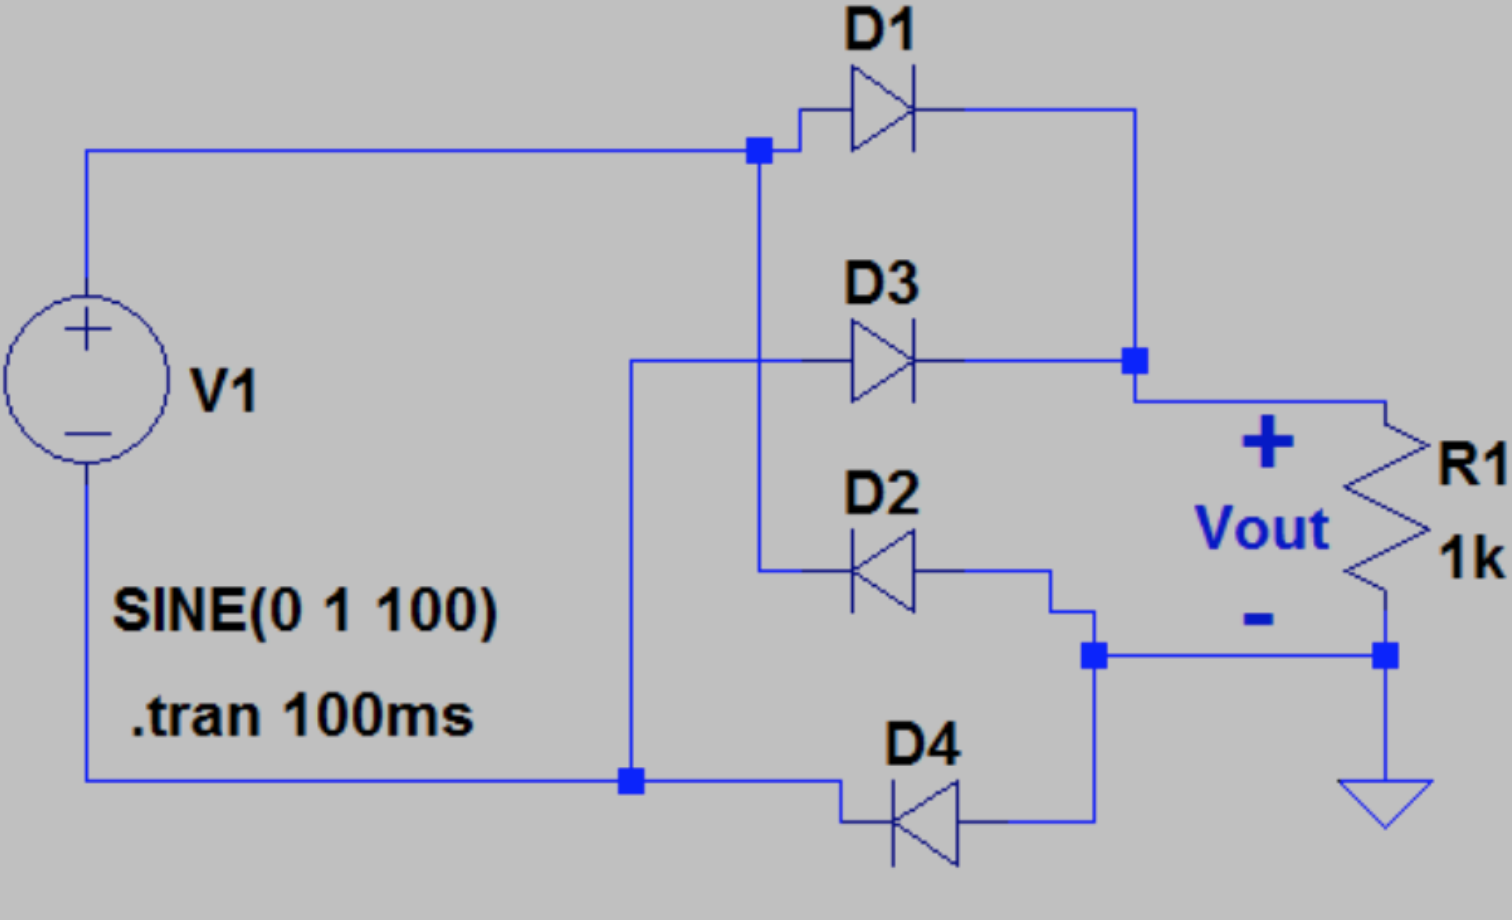
\includegraphics[width=.8\linewidth]{Figures/YILMAZ_silicon_diode_rectifier}  
		\caption{Rectificador basado en diodos de silicio}
		\label{fig:rect_diodos}
	\end{subfigure}
	\begin{subfigure}{.5\textwidth}
		\centering
		% include second image
		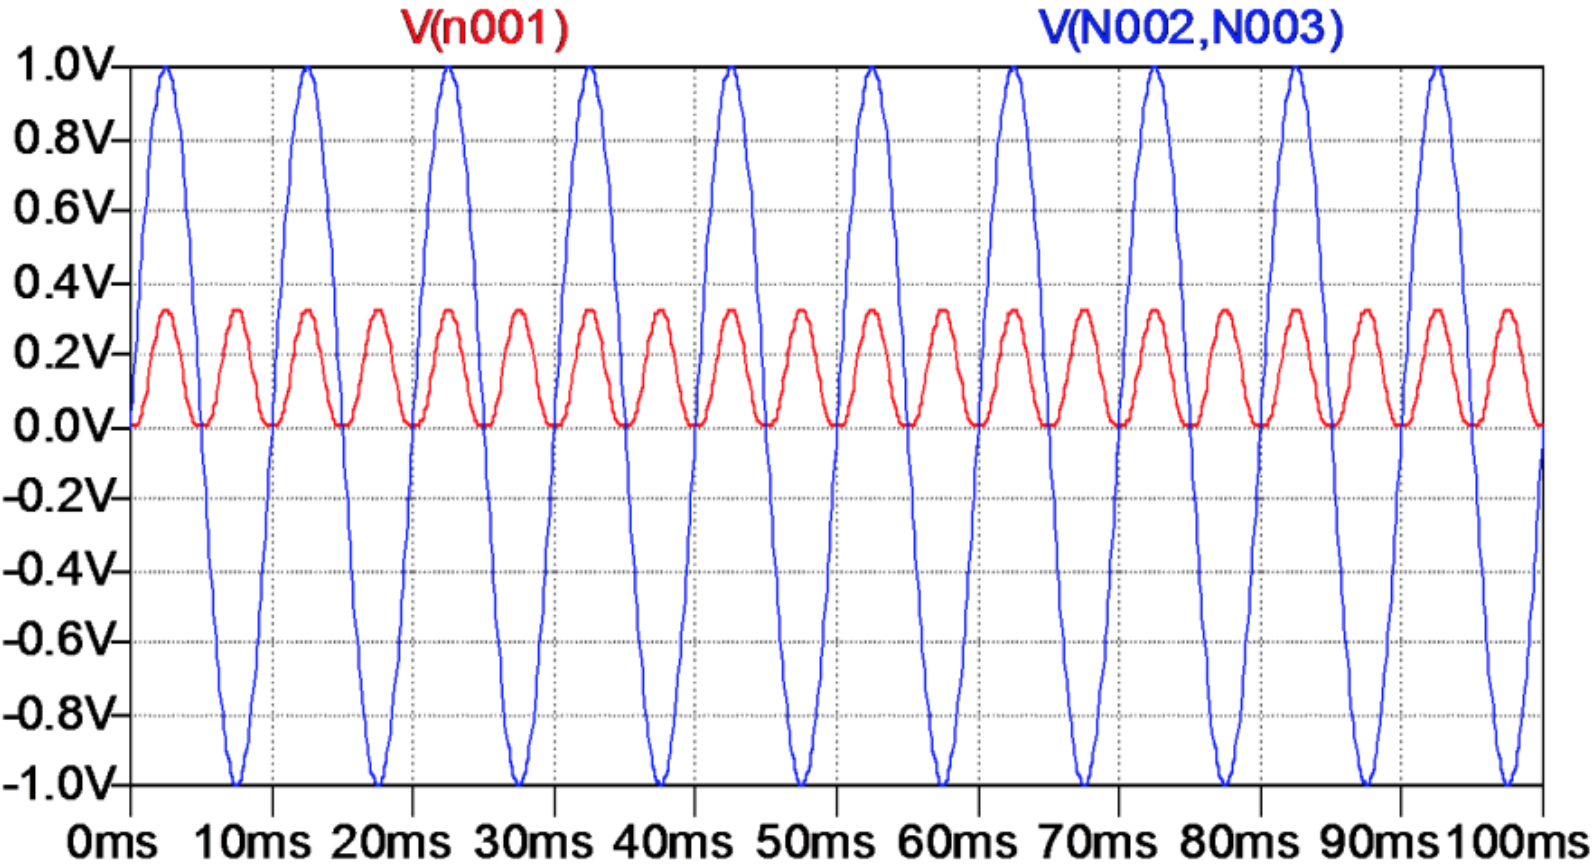
\includegraphics[width=.8\linewidth]{Figures/onda_silicon_rectifier}  
		\caption{Caída de tensión generada por el rectificador de la figura \ref{fig:rect_diodos}}
		\label{fig:onda_rectificador_diodos}
	\end{subfigure}
	\newline
	\begin{subfigure}{.5\textwidth}
		\centering
		% include third image
		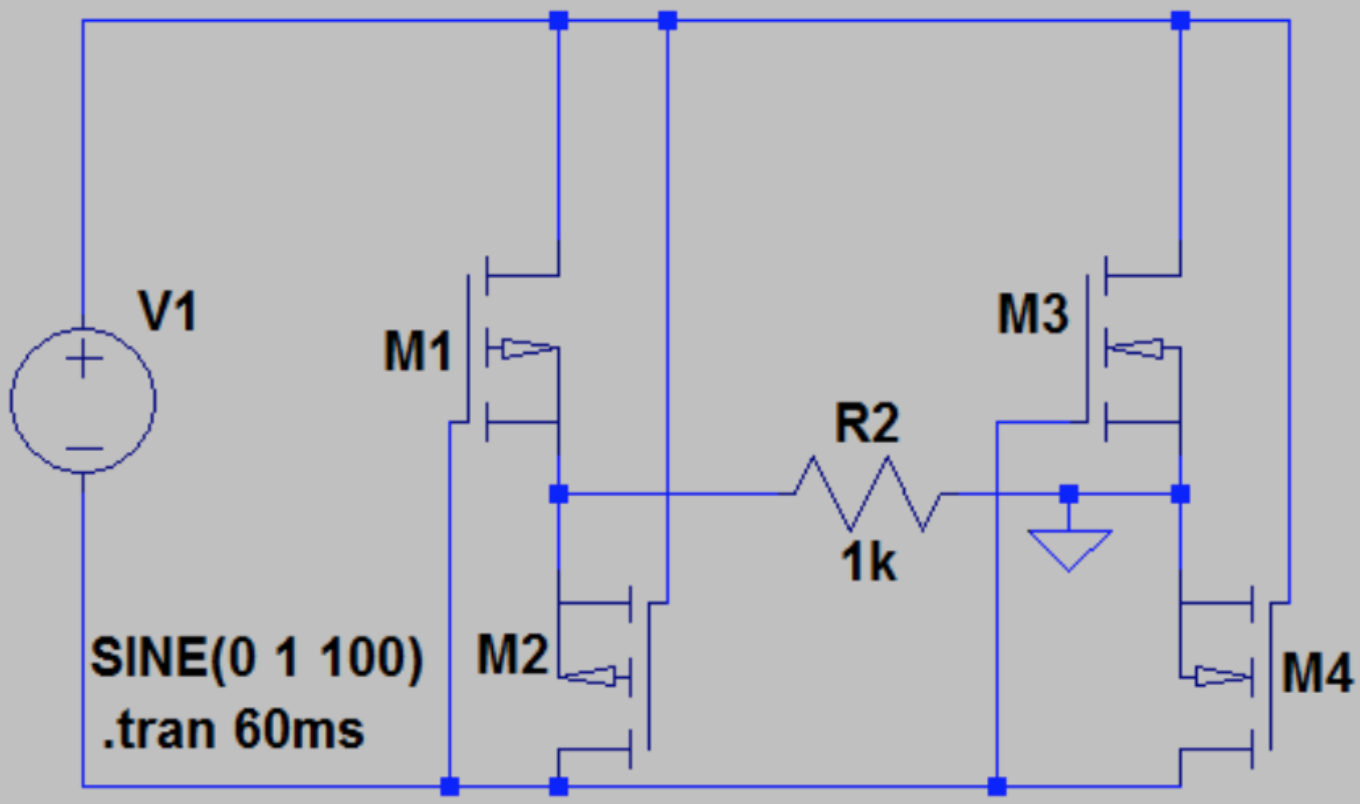
\includegraphics[width=.8\linewidth]{Figures/YILMAZ_passive_MOSFET_rectifier}  
		\caption{Rectificador basado en transistores MOSFET}
		\label{fig:rect_MOSFET}
	\end{subfigure}
	\begin{subfigure}{.5\textwidth}
		\centering
		% include fourth image
		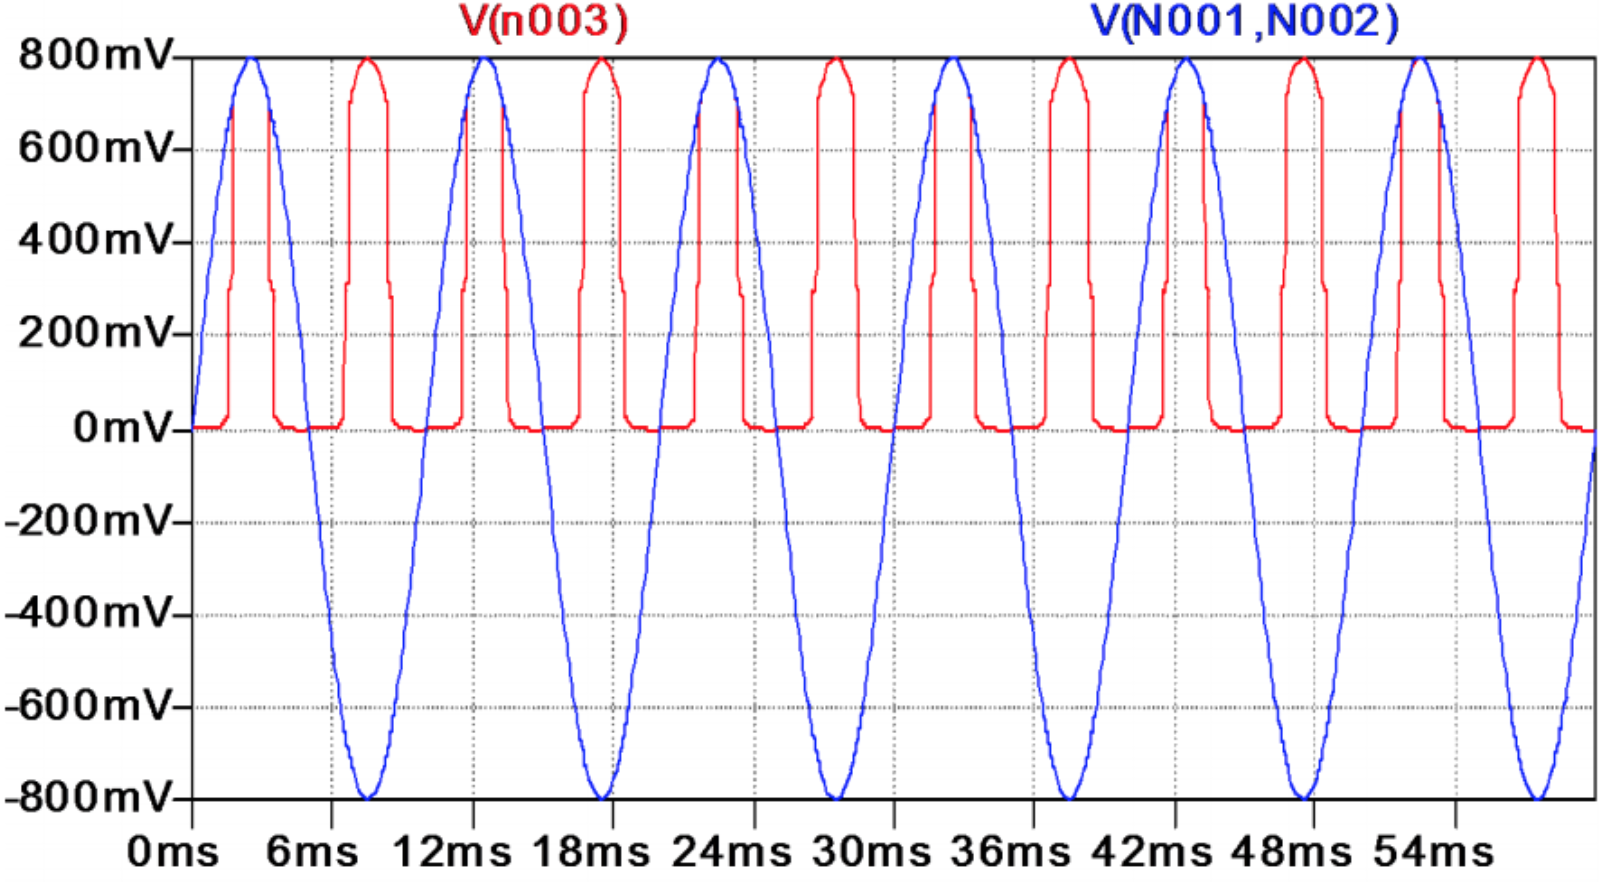
\includegraphics[width=.8\linewidth]{Figures/onda_passive_mosfet_rectifier}  
		\caption{Caída de tensión generada por el rectificador de la figura \ref{fig:rect_MOSFET}}
		\label{fig:onda_rectificador_MOSFET}
	\end{subfigure}
	\caption{Simulación de rectificadores basados en diodos y MOSFET. Imágenes tomadas de: \citep{Yilmaz}}
	\label{fig:comparacion_diodos_vs_MOSFET}
\end{figure}


\subsection{Supercapacitor como acumulador de energía}
La decisión de optar por un banco de supercapacitores (SC) como reemplazo total de una batería, se basa principalmente en el entorno donde operará el nodo HW. Diferencias entre una batería y un SC de interés para este proyecto, se plasman en la tabla \ref{tab:batteria_vs_supercap}.\\
Datos meteorológicos de la provincia de Misiones presentados en \citep{historico_temperaturas}, acusan temperaturas por encima de 30 C durante el periodo de septiembre a marzo. A diferencia de un SC que posee un rango de temperaturas de operación desde los -40 C hasta 70 C \citep{datasheet_supercap}, condiciones por encima de 35 grados son nocivas para una batería y generan el deterioro prematuro de sus componentes\citep{MA2018653}.\\
Es importante remarcar que la densidad de energía que pueden almacenar también es diferente, una batería tiene una densidad de energía 60 veces mayor que un SC. Sin embargo, para esta aplicacion puntual no represento un factor importante a la hora de elegir el acumulador.\\
Por ultimo, en ciclo carga es mas complejo en el caso de una batería. Las etapas de su curva de carga deben ser respetados según sean a corriente o tensión constante. Esto trae acarreado implementar una electrónica adicional encargada de gestiónar estos 2 parámetros. En un capacitor, la curva de carga está definida por un circuito RC serie \citep{ceraolo2014fundamentals}.\\ 
\begin{table}
	\centering
	\caption{Comparativa entre una batería y un supercapacitor para este proyecto}
	\begin{tabular}{lcc} 
		\hline
		\multicolumn{1}{c}{}                                                  & Batería         & Supercapacitor                                                                         \\ 
		\hline
		\begin{tabular}[c]{@{}l@{}}Densidad de \\energía (Wh/Kg)\end{tabular} & 265             & 3.9                                                                                    \\
		\begin{tabular}[c]{@{}l@{}}Rango de \\temperatura (C)\end{tabular}    & 15 a 35         & -40 a 70                                                                               \\
		Gestión de carga                                                      & V o I constante & \begin{tabular}[c]{@{}c@{}}Determinado por un\\circuito RC serie \citep{ceraolo2014fundamentals}\end{tabular}  \\
		\hline
	\end{tabular}
	\label{tab:batteria_vs_supercap}
\end{table}

\subsection{Uso de mayúscula inicial para los título de secciones}
Si en el texto se hace alusión a diferentes partes del trabajo referirse a ellas como capítulo, sección o subsección según corresponda. Por ejemplo: ``En el capítulo \ref{Chapter1} se explica tal cosa'', o ``En la sección \ref{sec:ejemplo} se presenta lo que sea'', o ``En la subsección \ref{subsec:ejemplo} se discute otra cosa''.

Cuando se quiere poner una lista tabulada, se hace así:

\begin{itemize}
	\item Este es el primer elemento de la lista.
	\item Este es el segundo elemento de la lista.
\end{itemize}

Notar el uso de las mayúsculas y el punto al final de cada elemento.

Si se desea poner una lista numerada el formato es este:

\begin{enumerate}
	\item Este es el primer elemento de la lista.
	\item Este es el segundo elemento de la lista.
\end{enumerate}

Notar el uso de las mayúsculas y el punto al final de cada elemento.

\subsection{Este es el título de una subsección}
\label{subsec:ejemplo}

Se recomienda no utilizar \textbf{texto en negritas} en ningún párrafo, ni tampoco texto \underline{subrayado}. En cambio sí se debe utilizar \textit{texto en itálicas} para palabras en un idioma extranjero, al menos la primera vez que aparecen en el texto. En el caso de palabras que estamos inventando se deben utilizar ``comillas'', así como también para citas textuales. Por ejemplo, un \textit{digital filter} es una especie de ``selector'' que permite separar ciertos componentes armónicos en particular.

La escritura debe ser impersonal. Por ejemplo, no utilizar ``el diseño del firmware lo hice de acuerdo con tal principio'', sino ``el firmware fue diseñado utilizando tal principio''. 

El trabajo es algo que al momento de escribir la memoria se supone que ya está concluido, entonces todo lo que se refiera a hacer el trabajo se narra en tiempo pasado, porque es algo que ya ocurrió. Por ejemplo, "se diseñó el firmware empleando la técnica de test driven development".

En cambio, la memoria es algo que está vivo cada vez que el lector la lee. Por eso transcurre siempre en tiempo presente, como por ejemplo:

``En el presente capítulo se da una visión global sobre las distintas pruebas realizadas y los resultados obtenidos. Se explica el modo en que fueron llevados a cabo los test unitarios y las pruebas del sistema''.

Se recomienda no utilizar una sección de glosario sino colocar la descripción de las abreviaturas como parte del mismo cuerpo del texto. Por ejemplo, RTOS (\textit{Real Time Operating System}, Sistema Operativo de Tiempo Real) o en caso de considerarlo apropiado mediante notas a pie de página.

Si se desea indicar alguna página web utilizar el siguiente formato de referencias bibliográficas, dónde las referencias se detallan en la sección de bibliografía de la memoria, utilizado el formato establecido por IEEE en \citep{IEEE:citation}. Por ejemplo, ``el presente trabajo se basa en la plataforma EDU-CIAA-NXP \citep{CIAA}, la cual...''.

\subsection{Figuras} 

Al insertar figuras en la memoria se deben considerar determinadas pautas. Para empezar, usar siempre tipografía claramente legible. Luego, tener claro que \textbf{es incorrecto} escribir por ejemplo esto: ``El diseño elegido es un cuadrado, como se ve en la siguiente figura:''

\begin{figure}[h]
\centering
\includegraphics[scale=.45]{./Figures/cuadradoAzul.png}
\end{figure}

La forma correcta de utilizar una figura es con referencias cruzadas, por ejemplo: ``Se eligió utilizar un cuadrado azul para el logo, como puede observarse en la figura \ref{fig:cuadradoAzul}''.

\begin{figure}[ht]
	\centering
	\includegraphics[scale=.45]{./Figures/cuadradoAzul.png}
	\caption{Ilustración del cuadrado azul que se eligió para el diseño del logo.}
	\label{fig:cuadradoAzul}
\end{figure}

El texto de las figuras debe estar siempre en español, excepto que se decida reproducir una figura original tomada de alguna referencia. En ese caso la referencia de la cual se tomó la figura debe ser indicada en el epígrafe de la figura e incluida como una nota al pie, como se ilustra en la figura \ref{fig:palabraIngles}.

\begin{figure}[htpb]
	\centering
	\includegraphics[scale=.3]{./Figures/word.jpeg}
	\caption{Imagen tomada de la página oficial del procesador\protect\footnotemark.}
	\label{fig:palabraIngles}
\end{figure}

\footnotetext{Imagen tomada de \url{https://goo.gl/images/i7C70w}}

La figura y el epígrafe deben conformar una unidad cuyo significado principal pueda ser comprendido por el lector sin necesidad de leer el cuerpo central de la memoria. Para eso es necesario que el epígrafe sea todo lo detallado que corresponda y si en la figura se utilizan abreviaturas entonces aclarar su significado en el epígrafe o en la misma figura.



\begin{figure}[ht]
	\centering
	\includegraphics[scale=.37]{./Figures/questionMark.png}
	\caption{¿Por qué de pronto aparece esta figura?}
	\label{fig:questionMark}
\end{figure}

Nunca colocar una figura en el documento antes de hacer la primera referencia a ella, como se ilustra con la figura \ref{fig:questionMark}, porque sino el lector no comprenderá por qué de pronto aparece la figura en el documento, lo que distraerá su atención.

Otra posibilidad es utilizar el entorno \textit{subfigure} para incluir más de una figura, como se puede ver en la figura \ref{fig:three graphs}. Notar que se pueden referenciar también las figuras internas individualmente de esta manera: \ref{fig:1de3}, \ref{fig:2de3} y \ref{fig:3de3}.
 
\begin{figure}[!htpb]
     \centering
     \begin{subfigure}[b]{0.3\textwidth}
         \centering
         \includegraphics[width=.65\textwidth]{./Figures/questionMark}
         \caption{Un caption.}
         \label{fig:1de3}
     \end{subfigure}
     \hfill
     \begin{subfigure}[b]{0.3\textwidth}
         \centering
         \includegraphics[width=.65\textwidth]{./Figures/questionMark}
         \caption{Otro.}
         \label{fig:2de3}
     \end{subfigure}
     \hfill
     \begin{subfigure}[b]{0.3\textwidth}
         \centering
         \includegraphics[width=.65\textwidth]{./Figures/questionMark}
         \caption{Y otro más.}
         \label{fig:3de3}
     \end{subfigure}
        \caption{Tres gráficos simples}
        \label{fig:three graphs}
\end{figure}

El código para generar las imágenes se encuentra disponible para su reutilización en el archivo \file{Chapter2.tex}.

\subsection{Tablas}

Para las tablas utilizar el mismo formato que para las figuras, sólo que el epígrafe se debe colocar arriba de la tabla, como se ilustra en la tabla \ref{tab:peces}. Observar que sólo algunas filas van con líneas visibles y notar el uso de las negritas para los encabezados.  La referencia se logra utilizando el comando \verb|\ref{<label>}| donde label debe estar definida dentro del entorno de la tabla.

\begin{verbatim}
\begin{table}[h]
	\centering
	\caption[caption corto]{caption largo más descriptivo}
	\begin{tabular}{l c c}    
		\toprule
		\textbf{Especie}     & \textbf{Tamaño} & \textbf{Valor}\\
		\midrule
		Amphiprion Ocellaris & 10 cm           & \$ 6.000 \\		
		Hepatus Blue Tang    & 15 cm           & \$ 7.000 \\
		Zebrasoma Xanthurus  & 12 cm           & \$ 6.800 \\
		\bottomrule
		\hline
	\end{tabular}
	\label{tab:peces}
\end{table}
\end{verbatim}


\begin{table}[h]
	\centering
	\caption[caption corto]{caption largo más descriptivo}
	\begin{tabular}{l c c}    
		\toprule
		\textbf{Especie} 	 & \textbf{Tamaño} 		& \textbf{Valor}  \\
		\midrule
		Amphiprion Ocellaris & 10 cm 				& \$ 6.000 \\		
		Hepatus Blue Tang	 & 15 cm				& \$ 7.000 \\
		Zebrasoma Xanthurus	 & 12 cm				& \$ 6.800 \\
		\bottomrule
		\hline
	\end{tabular}
	\label{tab:peces}
\end{table}

En cada capítulo se debe reiniciar el número de conteo de las figuras y las tablas, por ejemplo, figura 2.1 o tabla 2.1, pero no se debe reiniciar el conteo en cada sección. Por suerte la plantilla se encarga de esto por nosotros.

\subsection{Ecuaciones}
\label{sec:Ecuaciones}

Al insertar ecuaciones en la memoria dentro de un entorno \textit{equation}, éstas se numeran en forma automática  y se pueden referir al igual que como se hace con las figuras y tablas, por ejemplo ver la ecuación \ref{eq:metric}.

\begin{equation}
	\label{eq:metric}
	ds^2 = c^2 dt^2 \left( \frac{d\sigma^2}{1-k\sigma^2} + \sigma^2\left[ d\theta^2 + \sin^2\theta d\phi^2 \right] \right)
\end{equation}
                                                        
Es importante tener presente que si bien las ecuaciones pueden ser referidas por su número, también es correcto utilizar los dos puntos, como por ejemplo ``la expresión matemática que describe este comportamiento es la siguiente:''

\begin{equation}
	\label{eq:schrodinger}
	\frac{\hbar^2}{2m}\nabla^2\Psi + V(\mathbf{r})\Psi = -i\hbar \frac{\partial\Psi}{\partial t}
\end{equation}

Para generar la ecuación \ref{eq:metric} se utilizó el siguiente código:

\begin{verbatim}
\begin{equation}
	\label{eq:metric}
	ds^2 = c^2 dt^2 \left( \frac{d\sigma^2}{1-k\sigma^2} + 
	\sigma^2\left[ d\theta^2 + 
	\sin^2\theta d\phi^2 \right] \right)
\end{equation}
\end{verbatim}

Y para la ecuación \ref{eq:schrodinger}:

\begin{verbatim}
\begin{equation}
	\label{eq:schrodinger}
	\frac{\hbar^2}{2m}\nabla^2\Psi + V(\mathbf{r})\Psi = 
	-i\hbar \frac{\partial\Psi}{\partial t}
\end{equation}

\end{verbatim}